%(BEGIN_QUESTION)
% Copyright 2009, Tony R. Kuphaldt, released under the Creative Commons Attribution License (v 1.0)
% This means you may do almost anything with this work of mine, so long as you give me proper credit

Bring the following materials to class to build your own four-wire conductivity probe.  Partner with several classmates ahead of time to bring these materials, and to perform the experiment together in class as a team:

\begin{itemize}
\item{} Four large paperclips 
\vskip 5pt
\item{} Masking tape
\vskip 5pt
\item{} Small drinking cup (to fill with water)
\vskip 5pt
\item{} One pencil or plastic (non-metal) pen
\vskip 5pt
\item{} At least five ``alligator clip'' jumper wires (only three if multimeter has test clips)
\vskip 5pt
\item{} One 6-volt or 9-volt battery
\vskip 5pt
\item{} Resistor between 10 k$\Omega$ and 100 k$\Omega$ in value
\vskip 5pt
\item{} One or more packets of table salt (from the cafeteria)
\vskip 5pt
\item{} Multimeter capable of measuring DC millivolts
\end{itemize}

Bend the paperclips so they are straight, then wrap them around the pencil or pen to form a four-electrode conductivity probe, with the electrode spacing narrow enough for all four electrodes to easily fit into the opening of the cup.  Fold a length of masking tape over the four wires to hold them in position, ensuring consistent spacing between the wires as the prove is used.  {\it Do not get the masking tape wet with the sample water}, or else all subsequent conductivity measurements will be affected by electrical conductance within the wet tape.  Be sure to use steel paperclips rather than copper wires, as steel is much less chemically reactive with saltwater than copper.

$$\includegraphics[width=15.5cm]{i04126x01.eps}$$

The large resistor in series with the battery forms a crude current source: current output by the battery will be relatively constant despite changes in water conductivity because the large series resistor value ``swamps out'' the relatively small amount of resistance presented by the saltwater.  Your results will not be nearly as good without the resistor in series!

\vskip 10pt

The instructor will take several cups and prepare random concentrations of saltwater, identifying each cup with a number written on the side.  Your team's job is to use your conductivity probe to rank each solution in order from {\it greatest conductivity} to {\it least conductivity}.  In order to minimize the ``traffic congestion'' of students at the cups, it is recommended that members from each team quickly insert their probe into each solution and gather the raw data (voltage measurements) for each numbered cup, then return to their seats to analyze the data and rank the solutions.  When your team has agreed on a ranking, write your ranked results (from greatest to least) on a piece of paper and prepare to present your findings to the class. 

\vskip 20pt \vbox{\hrule \hbox{\strut \vrule{} {\bf Suggestions for Socratic discussion} \vrule} \hrule}

\begin{itemize}
\item{} Explain how this 4-wire conductivity probe design is similar to the design of a 4-wire RTD temperature sensor.  What is the purpose of using 4 wires instead of 2 wires in an RTD circuit, and how is this purpose similar to that in a 4-wire conductivity probe?
\item{} Explain how your conductivity instrument's response will be affected by increasing the spacing between all four electrodes.
\item{} Suppose we actually wished to {\it calibrate} a student-built conductivity probe so it measured solution conductivity in Siemens per centimeter.  How would we go about calibrating it to ensure it read conductivity accurately?
\end{itemize}

\underbar{file i04126}
%(END_QUESTION)





%(BEGIN_ANSWER)


%(END_ANSWER)





%(BEGIN_NOTES)

With the four-wire probe, the multimeter will register a lesser voltage as conductivity increases.  Distilled water will give the highest voltage readings, due to its very low conductivity.

\vskip 10pt

I recommend sparingly adding salt to the water.  No more than 1 cafeteria packet of salt to a cup of warm water.  Less is better.

\vskip 10pt

Here is some data taken from six student-built probes testing in class:

% No blank lines allowed between lines of an \halign structure!
% I use comments (%) instead, so that TeX doesn't choke.

$$\vbox{\offinterlineskip
\halign{\strut
\vrule \quad\hfil # \ \hfil & 
\vrule \quad\hfil # \ \hfil & 
\vrule \quad\hfil # \ \hfil \vrule \cr
\noalign{\hrule}
%
% First row
{\bf Unsalted} & {\bf 1 packet of salt} & {\bf 2 packets of salt} \cr
%
\noalign{\hrule}
%
% Another row
500 mV & 300 mV & 70 mV \cr
%
\noalign{\hrule}
%
% Another row
130 mV & 110 mV & 5 mV \cr
%
\noalign{\hrule}
%
% Another row
510 mV & 280 mV & 31 mV \cr
%
\noalign{\hrule}
%
% Another row
405 mV & 340 mV & 75 mV \cr
%
\noalign{\hrule}
%
% Another row
450 mV & 300 mV & 60 mV \cr
%
\noalign{\hrule}
%
% Another row
430 mV & 60 mV & 15 mV \cr
%
\noalign{\hrule}
} % End of \halign 
}$$ % End of \vbox

%INDEX% Chemistry, electrolysis of saltwater

%(END_NOTES)


